\chapter{Domain Driven Design}
\label{ch:ddd} %Label of the chapter lit rev. The key ``ch:lit_rev'' can be used with command \ref{ch:lit_rev} to refer this Chapter.

\section{Knowledge session for the exploration of the problem space}
\newpage
\section{Ubiquitos Language}
\begin{table}[!ht]
    \centering
    \begin{adjustbox}{max width=1.1\textwidth,center}
    \begin{tabular}{|l|p{10cm}|l|}
    \hline
        Nome & Descrizione & Sinonimi \\ \hline
        Mano & Distribuzione delle 40 carte ai 4 giocatori e la seguente serie di 10 prese & Round \\ \hline
        Mano & Carte dei giocatori non ancora giocate & Hand \\ \hline
        Presa & Quando ogni giocatore, a turno, gioca sul tavolo una carta. L’ultima presa della mano vale 1 punto. & Trick \\ \hline
        Partita & Insieme di più mani fino al raggiungimento del punteggio di 41 punti. & Game \\ \hline
        Partita corta & Insieme di più mani fino al raggiungimento del punteggio di 31 punti. & Short Game \\ \hline
        Tavolo & Raggruppamento di 4 giocatori, suddivisi in 2 coppie, i giocatori delle stessa squadra “siedono” in direzione opposta & Table \\ \hline
        Seme & Tipologia distintiva di carta, ne esistono 4: Denari, Coppe, Spade, Bastoni & Suit: Coins, Cups, Swords, Clubs~ \\ \hline
        Briscola & Seme con priorita’ piu’ alta. & Trump \\ \hline
        Maraffa & Se un giocatore possiede le tre carte di valore maggiore (asso, due e tre, dette assieme "Maraffa" o "Cricca")
        del seme di briscola, vince tre punti addizionali. In questo caso deve scendere con l'asso di quel seme. & Cricca, Marafon, Tresette con la Briscola \\ \hline
        Mazzo & 40 carte, di 4 semi diversi, 1,2,3,4,5,6,7, fante, cavallo e re. & Deck \\ \hline
        Taglio & Durante una mano in un seme viene giocato il seme di briscola, che avendo priorita’ maggiore
        permette di prendere nonostante il seme di gioco & Cut \\ \hline
        Busso & Invita il compagno, se possibile, a conquistare la presa e ad aprire il turno successivo con lo stesso seme & Knock \\ \hline
        Striscio corto & Quando si ha ancora in mano un basso numero di carte dello stesso seme con cui si è aperto il turno. & Short strip \\ \hline
        Striscio lungo & Quando si ha ancora in mano molte carte dello stesso seme con cui si è aperto il turno. & Long strip \\ \hline
        Volo & Quando non si hanno più carte del seme con cui si è aperto il turno. & Fly \\ \hline
        Figura & Fante, Cavallo, Re, con punteggio di 1/3 di punto. & Figure \\ \hline
        Asso & Carta con valore di 1 punto. & Ace \\ \hline
        Due e Tre & Carte con valore 1/3 di punto. & Two and Three \\ \hline
        Carta Liscia & Carte con numeri 4, 5, 6, 7. Sono prive di valore & Smooth paper \\ \hline
        Squadra & Coppie di giocatori seduti opposti & Team \\ \hline
        Giocatore & Persona che interagisce con l’applicativo & Player, User \\ \hline
        Chiamata fuori & Se un giocatore pensa che la sua squadra abbia raggiunto i 41 punti (o 31 punti nella variante "corta" della partita), la squadra può  dichiarare di avere già nel mazzo delle prese i punti per vincere e chiudere in anticipo l'ultima partita. In questo modo la mano termina immediatamente, senza che vengano giocate le restanti prese e la squadra che si è "chiamata fuori" impedisce all'altra squadra di conquistare ulteriori prese. Se una squadra si chiama fuori e, dopo aver contato i punti delle prese effettuate ed averli sommati ai punti ottenuti nelle mani già giocate, non raggiunge i punti per la vittoria (in gergo "sbaglia la chiamata") scatta automatico l'11 a 0 per la squadra avversaria & Call out \\ \hline
    \end{tabular}
    \end{adjustbox}
\end{table}
\newpage
\section{Bounded Context}
\section{Requisiti e casi d'uso}
\subsection{Requisiti}
\subsection{Scenario}
Si riporta di seguito lo schema dei casi d'uso che modella l'interazione dell'utente con l'applicazione.
\begin{figure}[h!]
\centering %increandire foto, troppo piccola
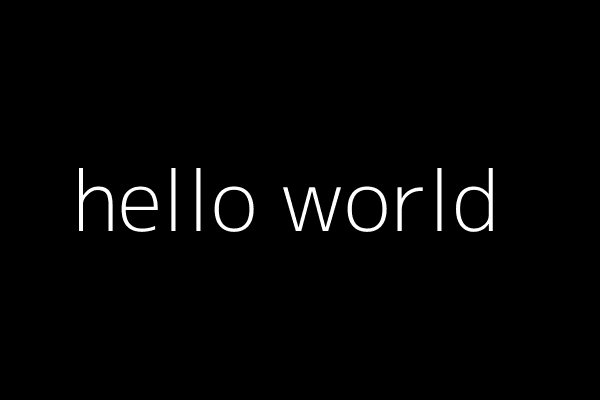
\includegraphics[scale=0.45]{assets\placeholder.png}
\caption{Schema dei casi d'uso}
\label{use_case}
\end{figure}
\subsection{Requirments}
\subsection{Casi d'uso}
\section{Riflessioni}
**Spiegare per quale motivo i pattern del DDD non sono stati applicati**
(shared kernel, publish consumer, ...)
